\newcommand{\bra}[1]{\langle #1|}
\newcommand{\ket}[1]{|#1\rangle}
\newcommand{\MET}{\slashed{E}_T}
\newcommand{\mDM}{m_{\rm{DM}}}
\newcommand{\mMed}{M_{\rm{med}}}
\newcommand{\gDM}{g_{\rm{DM}}}
\newcommand{\gq}{g_q}
\paragraph{Vector and axial vector mediator, s-channel exchange}

\begin{itemize}
\item Matrix Element implementations (with references)
\begin{itemize}
 \item Production mechanism
\begin{figure*}[t!]
\centering
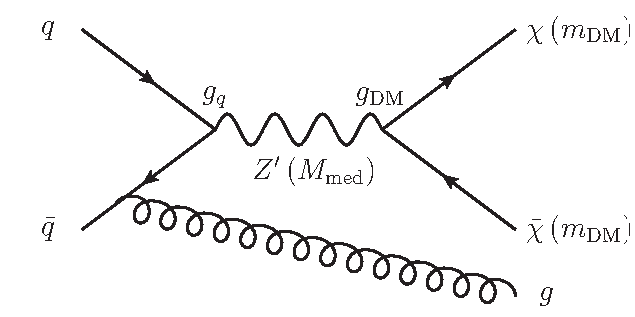
\includegraphics[width=0.5\linewidth]{figures/monoLHC.pdf}
\caption[][\baselineskip]{The diagram shows the pair production of dark matter particles in association with a parton from the initial state via an s-channel vector or axial-vector mediator. The process if specified by ($\mMed ,\, \mDM ,\, \gDM ,\, \gq)$, the mediator and dark matter masses, and the mediator couplings to dark matter and quarks respectively.}
\label{fig:OP}
\end{figure*}


 \item Lagrangian
We consider the case of a dark matter particle that is a Dirac fermion and where the production proceeds via the exhange of a spin-1 $s$-channel mediator. We consider the following interactions between the DM and SM fields including a vector mediator with:\\
(a) vector couplings to DM and SM.\\
(b) axial-vector couplings to DM and SM.\\

\begin{align}
\label{eq:AV} 
\mathcal{L}_{\mathrm{vector}} &= \sum_q \gq Z'_{\mu} \bar{q}\gamma^{\mu}q + \gDM Z'_{\mu} \bar{\chi}\gamma^{\mu}\chi \\
\mathcal{L}_{\rm{axial}} &= \sum_q \gq Z'_{\mu} \bar{q}\gamma^{\mu}\gamma^5q + \gDM Z'_{\mu} \bar{\chi}\gamma^{\mu}\gamma^5\chi
\end{align}
where the coupling extends over all the quarks and universal couplings are assumed for all the quarks. 
It is also possible to consider another model in which mixed vector and axial-vector couplings are considered, for instance the couplings to the quarks are vector whereas those to DM are axial-vector. As a starting point, we consider only the models with the vector couplings only and axial vector couplings only. Studies have been performed to see if the case of a mixed coupling can be simply extracted from the other models by some reweighting procedure to take account of the difference in cross section. This would assume that the difference between the pure and mixed couplings case does not affect the kinematics of the event. 


 \item Definition of minimal width
We assume that no additional visible or invisible decays contribute to the width of the mediator, this is referred to as the minimal width and it is defined as follows for the vector and axial-vector models.

\begin{equation}
\Gamma_{\rm{min}}=\Gamma_{\bar{\chi}\chi} + \sum_{q}N_{c}\Gamma_{\bar{q}q}
\end{equation}

where the individual contributions to this from the partial width are from,
\begin{align}
\Gamma_{\bar{\chi}\chi}^{\rm{vector}}&=\frac{\gDM^2 \mMed}{12\pi}\left(1+\frac{2 \mDM^2}{\mMed^2} \right)\sqrt{1-\frac{4 \mDM^2}{\mMed^2}}\\
\Gamma_{\bar{q}q}^{\rm{vector}}&= \frac{3 \gq^2 \mMed}{12\pi}\left(1+\frac{2 m_q^2}{\mMed^2} \right)\sqrt{1-\frac{4 m_q^2}{\mMed^2}}\\
\Gamma_{\bar{\chi}\chi}^{\rm{axial}}&=\frac{\gDM^2 \mMed}{12\pi} \left(1-\frac{4 \mDM^2}{\mMed^2}\right)^{3/2}\\
\Gamma_{\bar{q}q}^{\rm{axial}}&= \frac{3 \gq^2 \mMed}{12\pi}\left(1-\frac{4 m_q^2}{\mMed^2}\right)^{3/2}\label{eq:Gamma4}\;.
\end{align}

\end{itemize}
\item Couplings
\item Parameter choices (for scan)
Vary mediator mass and DM mass 
\item Generator implementation
There are several matrix element implementations of the s-channel vector mediated DM production. This is available in POWHEG, MADGRAPH and also MCFM.
The implementation in POWHEG generates DM pair production with 1 parton at Next-to-Leading-Order, whilst Madgraph and MCFM are at leading order. As shown in POWHEG paper{Haisch:2013ata}, including NLO corrections result in an enhancement in the cross section as compared to leading-order (LO) and though this is not significant, it does lead to a substantial reduction in the dependence on the choice of the renormalisation and factorisation scale and hence the theoretical uncertainty on the signal prediction. 
Since NLO calculations are available for the process in POWHEG, we recommend to proceed with POWHEG as the generator of choice. 
In addition to this, studies conducted within the DM forum have shown that POWHEG is more efficient for the generation of events all the way out to the tails of the kinematic distributions (https://indico.cern.ch/event/374678/session/0/material/3/1.pdf). 
The input configuration in POWHEG allows you to set parameters to not generate events below a given $k{T}$ cut ('bornktmin') and an additional parameter that ensures sufficient statistics at high transverse momentum ('bornsuppfact). With these flags set to appropriate variables, it is then possible to use a single POWHEG sample to generate the Monte Carlo for all signal regions, whereas with Madgraph more individual samples to be stitched together to achieve the required statistics out to the tails of the kinematic distributions. 
The POWHEG and Madgraph implementations were compared and the yields obtained from both were found to be compatible.  
\end{itemize}

\paragraph{Scalar and pseudoscalar mediator, s-channel exchange}

\paragraph{Colored scalar mediator, t-channel exchange}

\input tex/TChannelModels.tex

